\documentclass{ctexart}
\usepackage[a4paper,top=2cm,bottom=2cm,left=3cm,right=3cm,marginparwidth=1.75cm]{geometry}
\usepackage{extarrows}

\usepackage{amsmath}
\usepackage{graphicx}
\usepackage[colorlinks=true, allcolors=blue]{hyperref}
\usepackage{CJKutf8}
\usepackage{CJKpunct}

\title{热效应}
\author{笙}

\begin{document}
\tableofcontents
\maketitle


\begin{abstract}
化学.选修一.热效应.
\end{abstract}

\section{反应热}

反应热($Q$)：\textbf{等温条件}下，化学反应体系向环境释放或吸收的热量

\subsection{实验：中和反应热的测定}

下图用于测定反应热的实验装置称为\textbf{量热计}。

\begin{figure}[h]
\centering
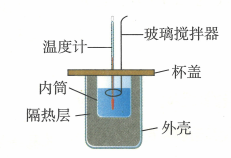
\includegraphics[width=0.5\linewidth]{Pic1.png}
\end{figure}

\subsubsection{实验原理}

一定量的$HCl$和$NaOH$溶液发生中和反应放出热量为$cm(t_2-t_1)$($c$：比热容；$m$：溶液体系质量；$t_2$、$t_1$：反应体系前后质量。

\subsubsection{实验步骤}

材料：$0.50mol/L$盐酸、$0.55mol/L$$NaOH$溶液。

步骤：

1.量筒量取$50ml$盐酸，倒入量热计内筒，插入温度计并测量温度。\textbf{用水冲洗干净温度计，擦干备用}。

2.另取量筒量取$50ml$$NaOH$溶液，用温度计测量温度。\textbf{用水冲洗干净温度计，擦干备用}。

3.重复上述步骤两次。

数据处理：填表，取三次测量所得温度差的均值作为计算数据。

\begin{figure}[h]
\centering
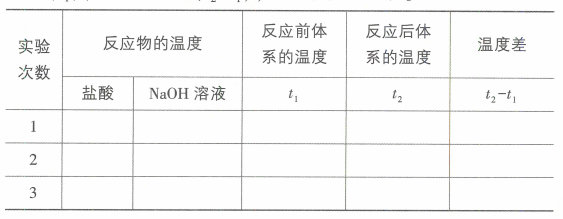
\includegraphics[width=0.8\linewidth]{Pic2.png}
\end{figure}

计算：根据公式计算得到生成$1mol H_2O$时放出的热量。

\subsection{反应热与焓变}

焓($H$)：与内能相关的物理量。

焓变($\Delta H$)：生成物总焓与反应物总焓之差， $\Delta H=H_2-H_1$($H_2$：生成物焓；$H_1$：反应物焓)。单位：$kJ/mol$。

Tips：焓变是与化学反应式一一对应的量，它的实际意义为“每摩尔反应”。

\subsubsection{反应热与焓变的关系}

对于\textbf{等压条件}下的化学反应，若反应中的物质能量全部转化为热能，则反应热等于反应的焓变。

\subsubsection{焓变的表示}

当反应体系放热时，焓减小，$\Delta H\textless 0$。

\subsubsection{反应过程与反应热的关系}

\begin{figure}[h]
\centering
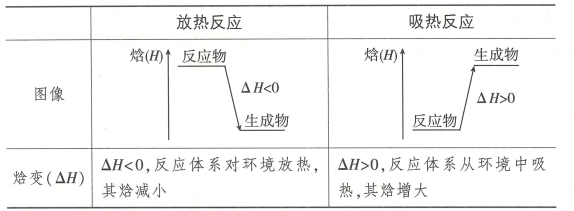
\includegraphics[width=0.8\linewidth]{Pic3.png}
\end{figure}

\subsubsection{微观角度理解化学反应中的能量变化}

\begin{figure}[h]
\centering
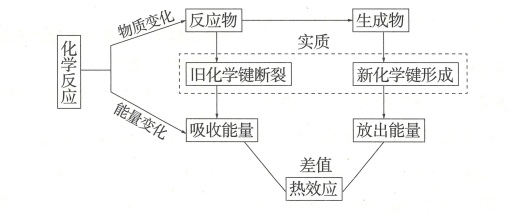
\includegraphics[width=0.8\linewidth]{Pic4.png}
\end{figure}

\newpage

\subsection{热化学方程式}

热化学方程式：用以表面反应释放或吸收热量的化学方程式。

\begin{equation*}
    \centering
    2H_2(g)+O_2(g)\xlongequal{}{} 2H_2O(l)\qquad\Delta H=-571.6kJ/mol
\end{equation*}

\subsubsection{书写要求}

1.注明反应时的室温和压强($25^{\circ}C$、$101kPa$可不注明)。

2.注明\textbf{反应物和生成物的状态}。固态：$s$；液态：$l$；气态：$g$；水溶液：$aq$。

3.化学计量数\textbf{只表示物质的物质的量}，可写成分数。

4.不需要标注气体和沉淀。

5.$\Delta H$和化学反应式一一对应，化学计量数加倍，$\Delta H$也加倍。

\subsubsection{深刻理解}

1.$\Delta H$和化学反应式一一对应。

2.对于可逆反应，$\Delta H$均表示按照化学计量数所表示的物质的量\textbf{完全反应}的反应热。

\begin{equation*}
    \centering
    2SO_2(g)+O_2(g)\rightleftharpoons{}{} 2SO_3(g)\qquad\Delta H=-197kJ/mol
\end{equation*}

对于上述反应，实际达到平衡时所放出的热量$Q\textless 197KJ$。

\subsection{燃烧热}

燃烧热：$101kPa$下，$1mol$纯物质燃烧所释放出的热量。单位：$kJ/mol$。燃烧热为\textbf{正}值，与焓变互为相反数。

完全燃烧生成制定产物：可燃物中$C$、$H$、$O$、$N$分别燃烧生成$CO_2(g)$、$H_2O(l)$、$O_2(g)$、$N_2(g)$。

和焓变一样，燃烧热的书写也与反应式一一对应。

\begin{equation*}
    \centering
    C_2H_2(g)+\frac{5}{2}O_2(g)\xlongequal{}{}2CO_2(g)+H_2O(l)\qquad \Delta H=-1299.6kJ/mol
\end{equation*}

\section{反应热的计算}

\subsection{盖斯定律}

盖斯定律：一个化学反应的反应热与反应步骤无关，\textbf{只与反应的始态和终态有关}。本质上是能量守恒定律。

\subsection{反应热的计算}

\subsubsection{依据热化学方程式(焓变)计算}

\begin{equation*}
    \centering
    S(g)+O_2(g)\xlongequal{}{}SO_2(g)\qquad\Delta H=-296.8kJ/mol
\end{equation*}

$Q$：$16g$固体硫完全燃烧释放多少热量？

\subsubsection{根据盖斯定律计算}

\begin{figure}[h]
\centering
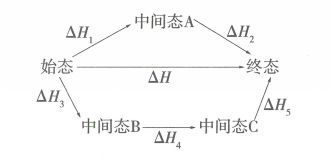
\includegraphics[width=0.6\linewidth]{Pic5.png}
\end{figure}

\begin{equation*}
    \centering
    \Delta H=\Delta H_1+\Delta H_2=\Delta H_3+\Delta H_4+\Delta H_5
\end{equation*}

\subsubsection{根据燃烧热计算}

方法等同焓变。

\subsubsection{根据化学键键能计算}

$\Delta H=$\textbf{反应物的化学键键能总和}$-$\textbf{生成物化学键键能总和}。

对于下述反应，$1mol$$H_2(g)$和$1molCl_2(g)$断裂化学键吸收能量$679KJ$，$2mol$$HCl(g)$生成新化学键释放能量$862KJ$。

\begin{equation*}
    H_2(g)+Cl_2(g)\xlongequal{}{}2HCl(g)\qquad\Delta H=?
\end{equation*}

\subsubsection{根据反应物和生成物总能量计算}

本质上是能量守恒定律。

\newpage

\subsubsection{根据图像计算}

\begin{figure}[h]
\centering
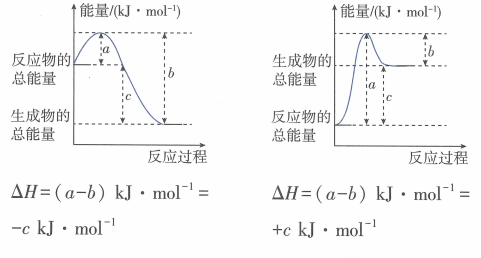
\includegraphics[width=0.8\linewidth]{Pic6.png}
\end{figure}

\subsection{反应热大小的比较}

为方便，下述反应均讨论放热反应。

\subsubsection{直接比较}

比较下述反应热大小。

\begin{equation*}
    \centering
    H_2(g)+\frac{1}{2}O_2(g)\xlongequal{}{}H_2O(l)\qquad\Delta H_1
\end{equation*}

\begin{equation*}
    \centering
    2H_2(g)+O_2(g)\xlongequal{}{}2H_2O(l)\qquad\Delta H_2
\end{equation*}

比较下述反应热大小。

\begin{equation*}
    \centering
    C(s)+\frac{1}{2}O_2(g)\xlongequal{}{}CO(g)\qquad\Delta H_1
\end{equation*}

\begin{equation*}
    \centering
    C(s)+O_2(g)\xlongequal{}{}CO_2(g)\qquad\Delta H_2
\end{equation*}

\subsubsection{盖斯定律比较法}

同一反应，\textbf{生成物状态不同}。

\begin{equation*}
    \centering
    A(g)+B(g)\xlongequal{}{}C(g)\qquad\Delta H_1
\end{equation*}

\begin{equation*}
    \centering
    A(g)+B(g)\xlongequal{}{}C(l)\qquad\Delta H_2
\end{equation*}

同一反应，\textbf{反应物状态不同}

\begin{equation*}
    \centering
    A(g)+B(g)\xlongequal{}{}C(g)\qquad\Delta H_1
\end{equation*}

\begin{equation*}
    \centering
    A(s)+B(g)\xlongequal{}{}C(g)\qquad\Delta H_2
\end{equation*}

\newpage

\subsubsection{图示比较法}

\begin{equation*}
    \centering
    S(g)+O_2(g)\xlongequal{}{}SO_2(g)\qquad\Delta H_1
\end{equation*}

\begin{equation*}
    \centering
    S(s)+O_2(g)\xlongequal{}{}SO_2(g)\qquad\Delta H_2
\end{equation*}

\begin{figure}[h]
\centering
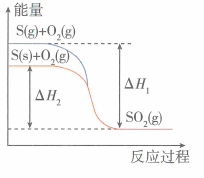
\includegraphics[width=0.5\linewidth]{Pic7.png}
\end{figure}


\end{document}